\section{Saddle Points}
\label{sec:sps}
Saddle points are stationary points, i.e. with zero gradient, on a multidimensional function, $f(\vR)$, that are neither maxima nor minima.

\begin{figure}[h]
  \begin{center}
  \subfigure[2D saddle point][2D saddle point, $f(x=0, y=0) = x^2 - y^2$. A minimum is the $x$-direction and a maximum in the $y$-direction]{
    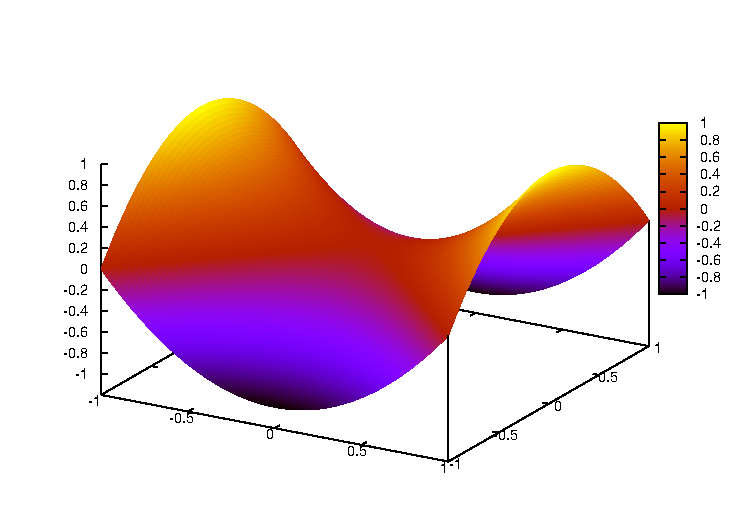
\includegraphics[width=0.6\linewidth]{saddle-point-2d}
    \label{fig:2d-saddle-point}
    }
  \subfigure[1D saddle point][1D saddle point, $f(x=0) = x^3$. Neither a maximum nor a minimum but the gradient is vanishing.]{
    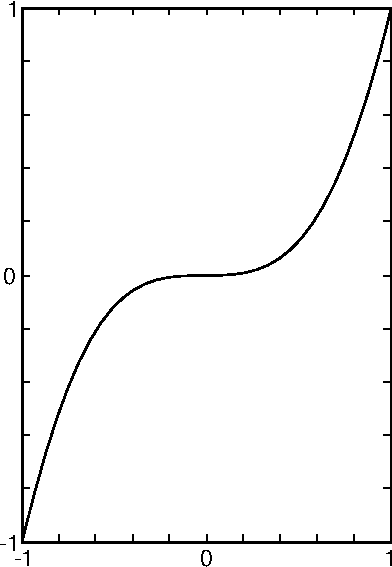
\includegraphics[width=0.26\linewidth]{saddle-point-1d}
    \label{fig:1d-saddle-point}
    }
    \parbox{0.85\linewidth}{
      \caption{Examples of first order saddle points.
      }
      \label{fig:saddle-points}
    }
  \end{center}
\end{figure}

A common view of a saddle (point) can be found in \fref{fig:2d-saddle-point}, as the function $f(x, y) = x^2 - y^2$ which near $(x,y) = (0,0)$ resembles a saddle, used when riding horses, curving upwards in one direction (along the horse) and downwards in the other (perpendicular to the horse).
This image of a saddle point lacks a few elements to tell their whole story but acts as a good general case.
On functions of higher dimensionality than $2$, different orders of saddle points are possible.
The order of the saddle point is decided by the amount of directions that are not at a minimum, or the non-positive eigenvalues of the Hessian.
As such, \fref{fig:2d-saddle-point} shows a first order saddle point on a two dimensional function.
In this thesis, saddle points of order $N$ will be indicated by \sap{N} from here on.

The Hessian at the \sap{} displayed in \fref{fig:2d-saddle-point} has one negative eigenvalue, however, a saddle point with one or more vanishing eigenvalues is also possible, such as the 1D example $f(x = 0) = x^3$, seen in \fref{fig:1d-saddle-point}.

Locating \sap{}s in multiple dimensions is a non-trivial task as only a limited number of steepest decent paths lead to each one while the majority lead to minima.
A number of schemes for locating \sap{1}s have been suggested (see~\cite{sp-mep-review-2002} for a review), out of which two popular ones are discussed in \fref{chap:saddle-point-methods}: The Dimer method and the Nudged Elastic Band method.
Furthermore, an extension to these methods for finding higher order \sap{}s is presented in \fref{chap:erm}.

In the context of atomic simulations, \sap{}s are important in describing reactions and reaction rates.
